\subsection{Сбор графа потока данных} \label{sec:dfg_collection}

Обозначим \gls{dfg_math} - граф потока данных, где $V$ \, - множество вершин графа, $E \subseteq V \times V$ \, - множество ребер графа. Так же обозначим: \gls{edges_subsets} \, - множество всех подмножеств ребер графа. Вершины графа соответствуют отдельным выполнениям инструкций и далее называются инструкциями. Ребра -- зависимости между инструкциями по данным. С каждым ребром ассоциируются значение и локация, по которой данное значение располагалось во время трассировки, например регистр или область памяти. Для представления графа потока данных используется реализация списка смежности из библиотеки boost graph (boost::adjacency\_list) \cite{boost_graph_library,boost_adjacency_list}.

Boost graph позволяет ассоциировать с вершинами и ребрами пользовательские данные. Для инструкций хранятся: номер (уникальный идентификатор) инструкции, адрес инструкции, ее код. Для ребер хранятся: восьми-байтное значение и его локация (уже упомянутые ранее) - в памяти или на регистре общего назначения, модификаторы значения: тип расширения, размеры битовых сдвигов, и т. п. Заметим, что размер значения фиксированный, зависимости по значениям большего размера отображаются с помощью нескольких ребер.

На графе есть вершины, не соответствующие реальным инструкциям (вершина "начальное состояние"\, на рис. \ref{fig:dfg_example}). Будем называть такие вершины \glsdisp{pseudo_source}{псевдо-инструкциями}. Такие вершины всегда являются истоками и используются для отображения зависимостей, не порождаемых отдельными инструкциями, или для добавления вспомогательных зависимостей:

\begin{itemize}
    \item Вершина начального состояния - для зависимостей от начального состояния памяти или начальных значений регистров.

    \item Вершина внешних зависимостей по памяти - для зависимостей по памяти, модифицированной другим потоком или ОС.

    Пример: Из памяти прочитано значение, не соответствующее текущему образу памяти. Данное значение могло быть записано другим потоком или ОС во время системного вызова или обработки системного исключения. На графе данная зависимость будет представлена в виде ребра, выходящего из вершины внешних зависимостей и входящего в инструкцию, прочитавшую новое значение.

    \item Вершина сложных зависимостей по памяти - для зависимостей по памяти от нескольких инструкций.

    В данный момент полноценная поддержка таких зависимостей отсутствует.
\end{itemize}

\begin{figure}[h!]
    \centering
    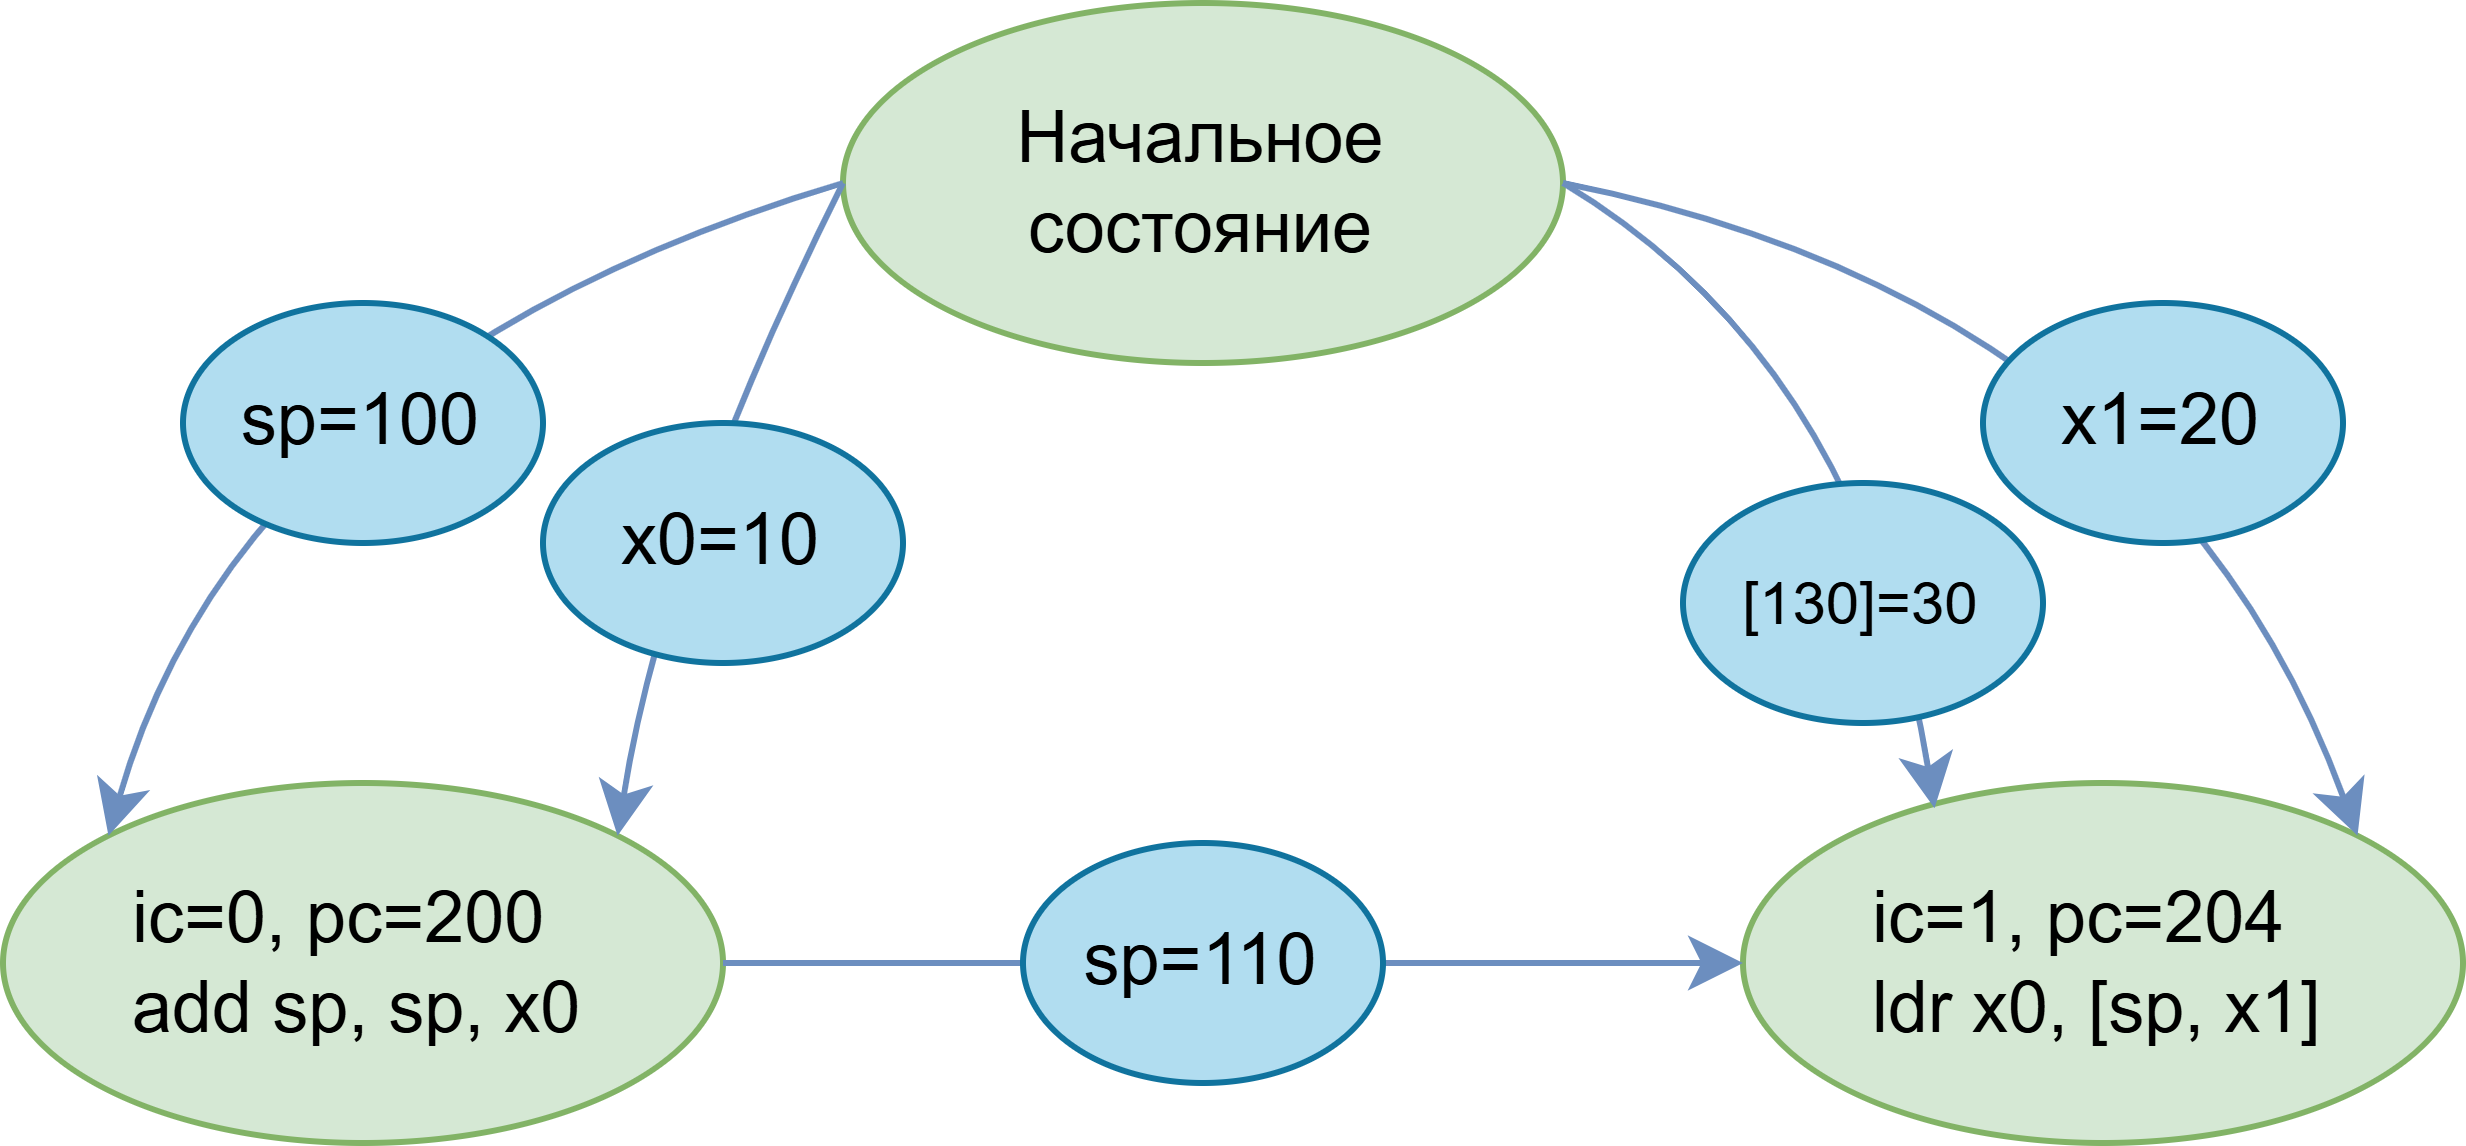
\includegraphics[width=0.7\linewidth]{pics/dfg_example.drawio.png}
    \caption{Пример графа потока данных.}
    \label{fig:dfg_example}
\end{figure}
\FloatBarrier

Сбор графа потока данных начинается с симуляционного прохода по трассе (блок схема алгоритма представлена на рис. \ref{fig:trace_simulation}), в ходе которого собираются:

\begin{itemize}
    \item Граф потока данных.
    \item Данные вершин.
    \item Данные ребер, кроме модификаторов значений (таких как размеры битовых сдвигов и т. п.).
    \item Карта, отображающая идентификаторы инструкций в дескрипторы, с помощью которых осуществляется доступ к вершинам.
    \item Карта зависимостей инструкций от флагов условий.
\end{itemize}

Заметим, что зависимости между инструкциями по флагам условий хранятся отдельно от графа потока данных. Данное решение позволяет разделить разнородные зависимости, что существенно упрощает обработку.

\begin{figure}[h!]
    \centering
    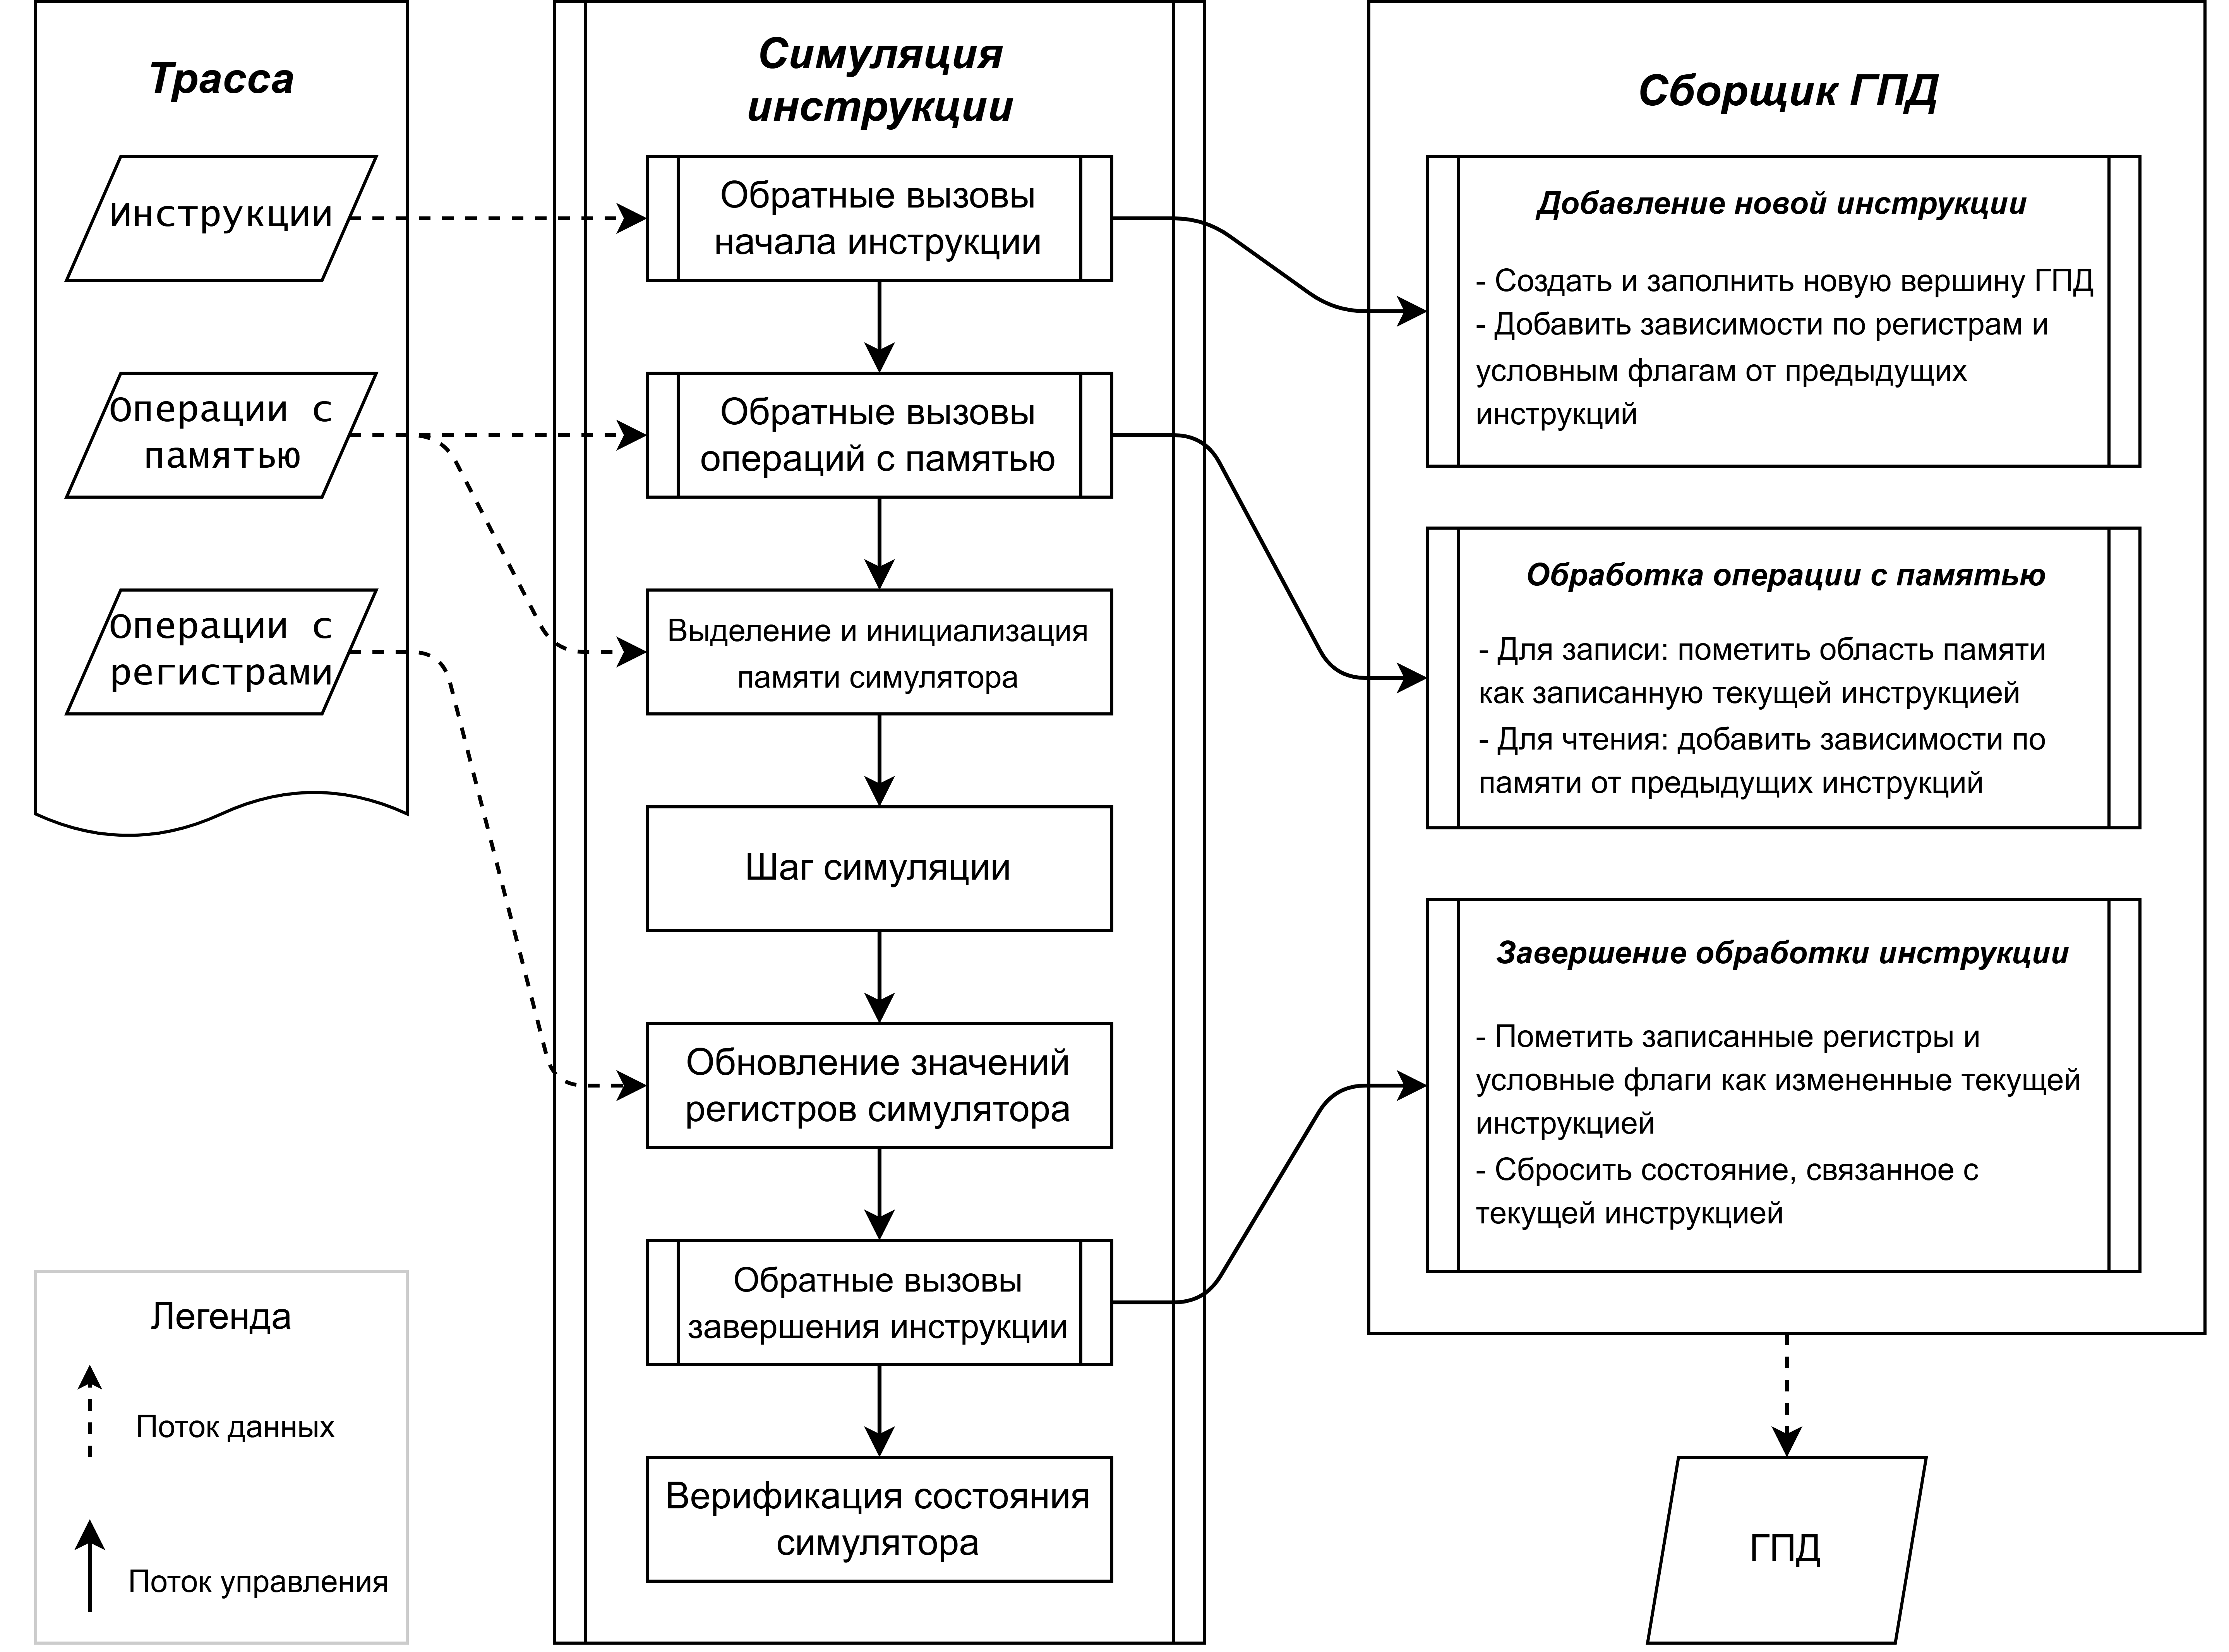
\includegraphics[width=0.8\linewidth]{pics/trace_simulation.drawio.png}
    \caption{Блок схема алгоритма симуляционного прохода по трассе.}
    \label{fig:trace_simulation}
\end{figure}
\FloatBarrier

После симуляционного прохода производится ряд обходов графа, в ходе которых собираются:

\begin{itemize}
    \item Карты подсказок для алгоритмов анализа адресов.
    \item Модификаторы значений для ребер графа.
\end{itemize}

Карты подсказок позволяют получать вспомогательные данные для вершин и ребер графа (примеры фрагментов ГПД и сформированных для них подсказок представлены на рис. \ref{fig:heuristics_hints}):

\begin{itemize}
    \item src\_edge\_hints : $E \rightarrow E$ \, задает порядок обратного обхода графа для алгоритма поиска адресов в ряде краевых случаев. Формируется с помощью набора эвристик.
    \item dst\_edge\_hints : $E \rightarrow 2^E = src\_edge\_hints^{-1}$ \, задает порядок прямого обхода графа для алгоритма поиска адресов в ряде краевых случаев. Задает обратное многозначное отображение для src\_edge\_hints.
    \item base\_edge\_hints : $V \rightarrow E$ \, отображает вершины в соответствующие им входные ребра базовых адресов.
    \item offset\_edge\_hints : $V \rightarrow E$ \, отображает вершины в соответствующие им входные ребра смещений адресов.
\end{itemize}

\begin{figure}[h!]
    \centering
    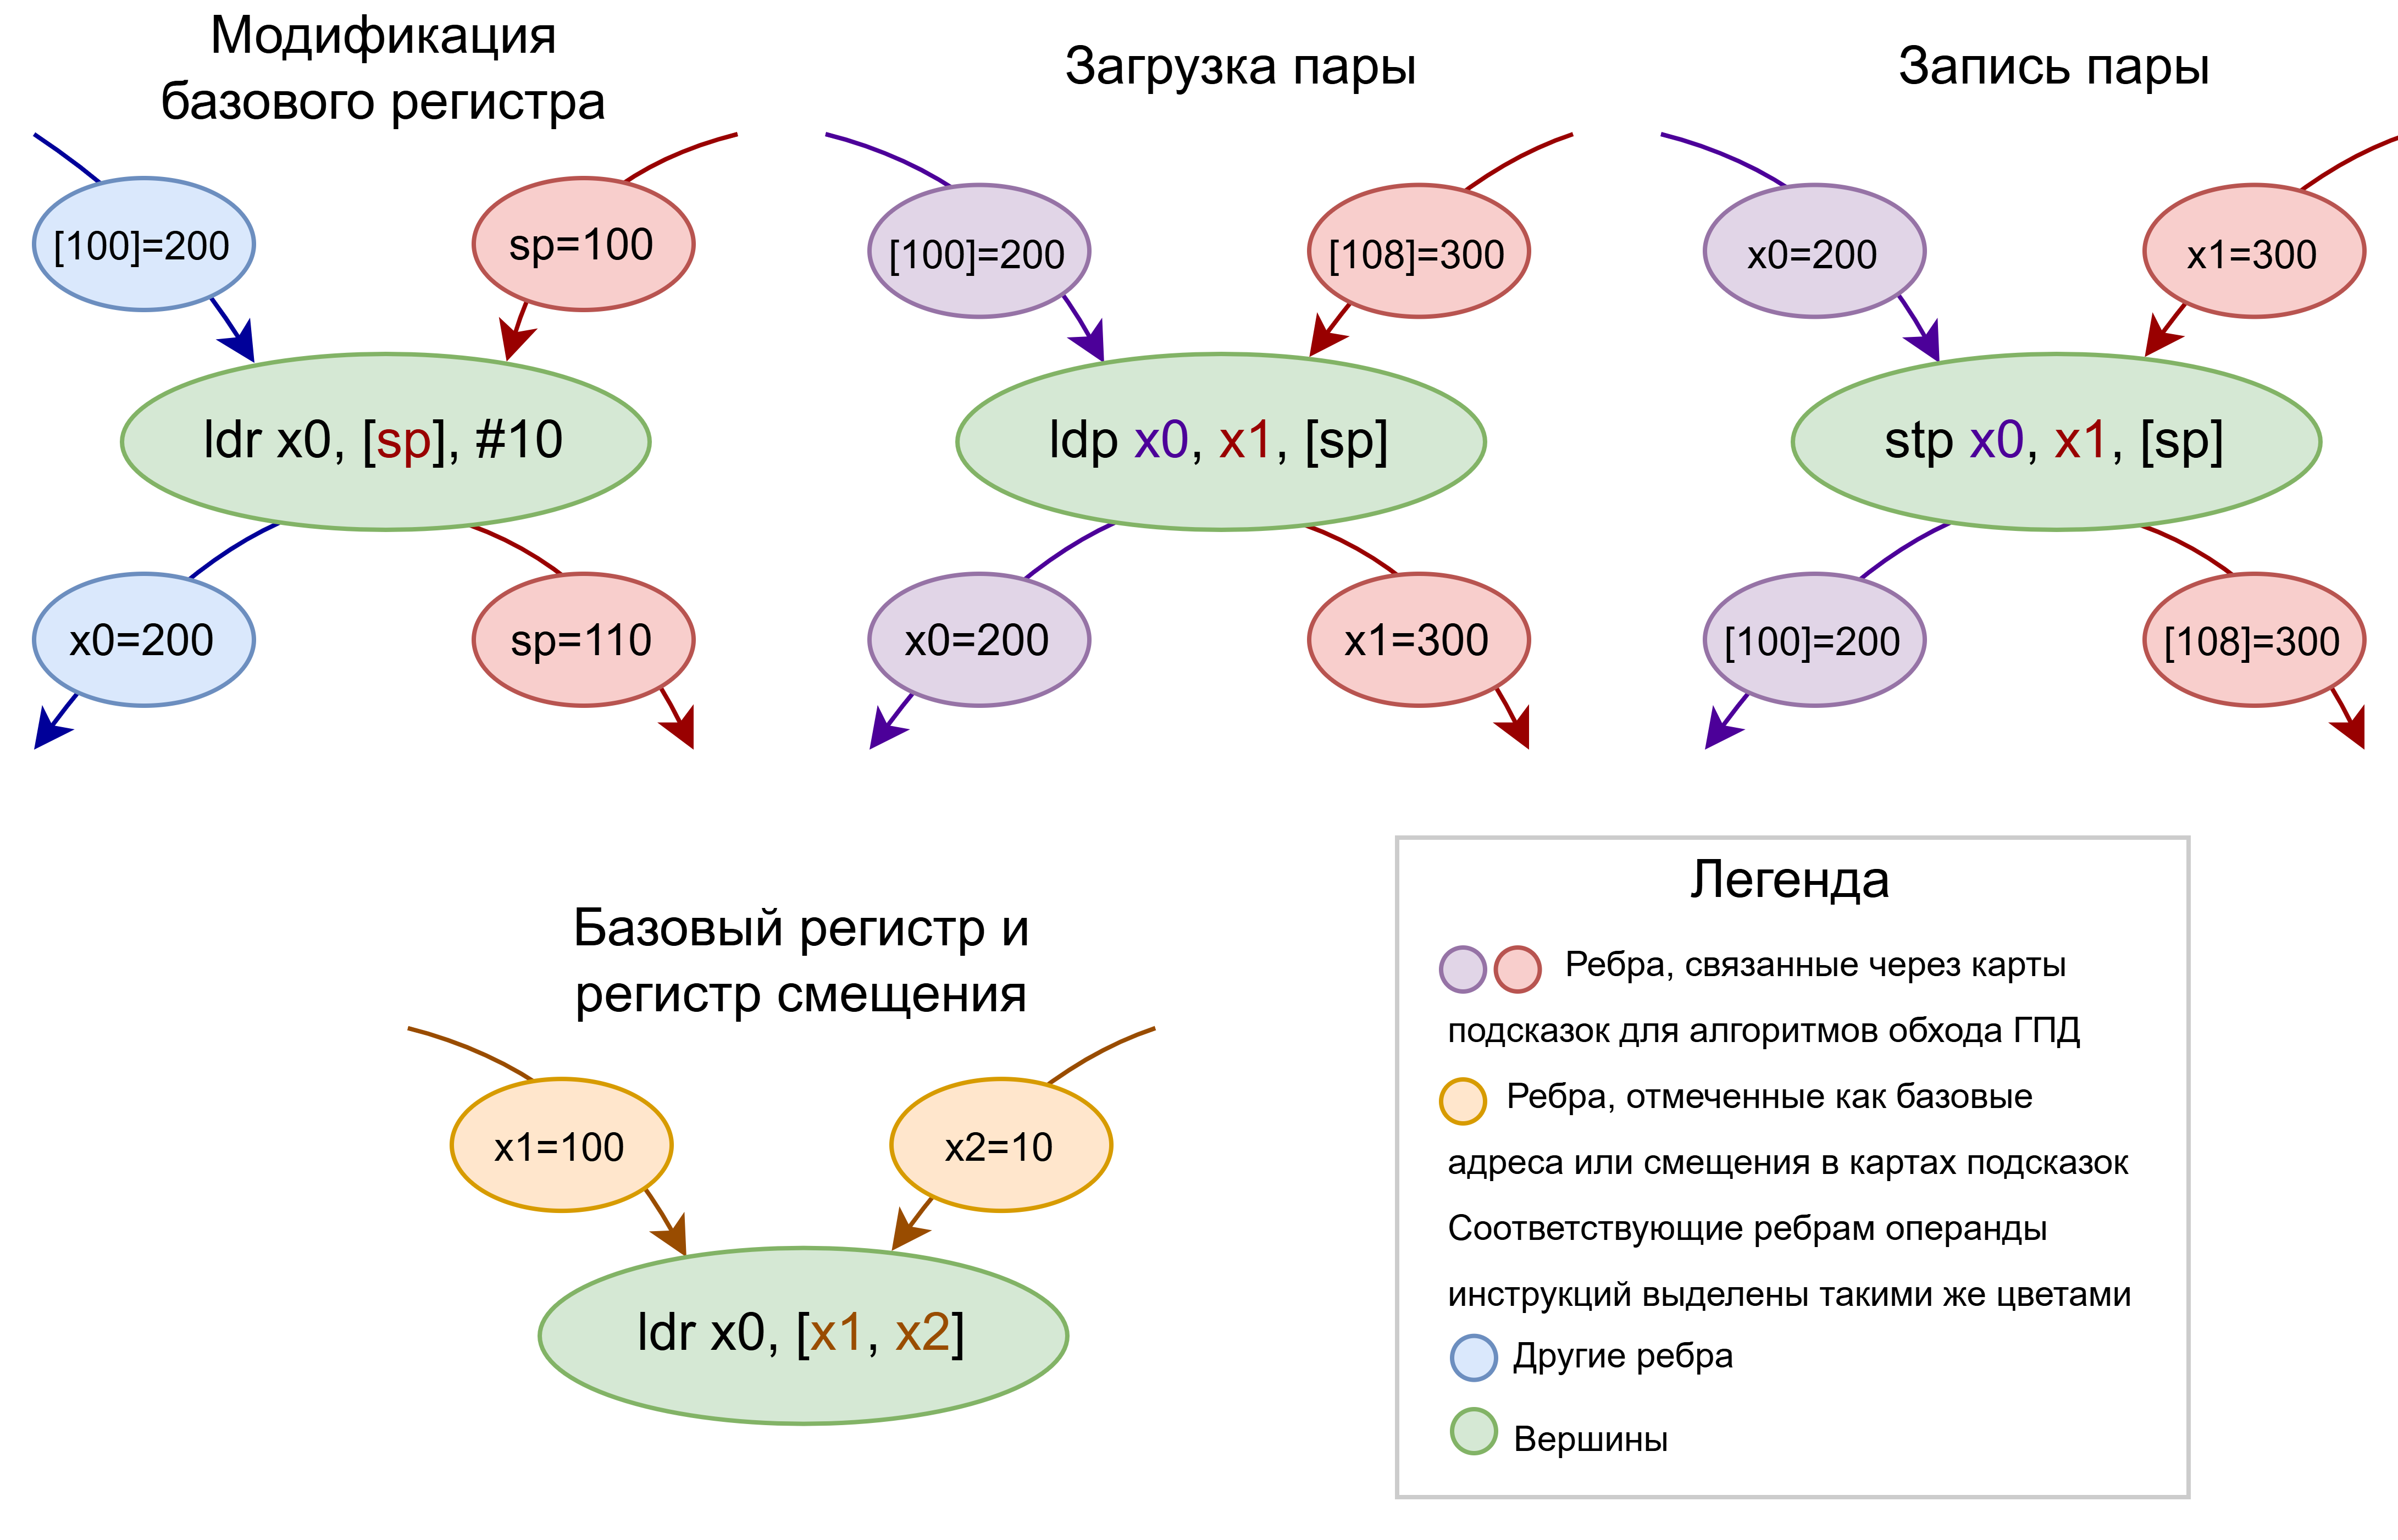
\includegraphics[width=0.8\linewidth]{pics/heuristics_hints.drawio.png}
    \caption{Примеры фрагментов ГПД и сформированных для них подсказок.}
    \label{fig:heuristics_hints}
\end{figure}

На рис. \ref{fig:dfg_uml} представлена UML диаграмма \cite{omg_uml_specification,selic_uml_overview} модуля, отвечающего за сбор и анализ графа потока данных (модуль ГПД).

\begin{figure}[h!]
    \centering
    \includegraphics[width=0.9\linewidth]{pics/dfg_uml.drawio.png}
    \caption{UML диаграмма модуля ГПД.}
    \label{fig:dfg_uml}
\end{figure}
\FloatBarrier
